\documentclass[12pt]{article}
\usepackage[margin=1in]{geometry} 
\usepackage{amsmath}
\usepackage{amssymb}
\usepackage{siunitx}
\usepackage{float}
\usepackage{tikz}
\def\checkmark{\tikz\fill[scale=0.4](0,.35) -- (.25,0) -- (1,.7) -- (.25,.15) -- cycle;} 
\usepackage{url}
\usepackage[siunitx,american,RPvoltages]{circuitikz}
\ctikzset{capacitors/scale=0.7}
\ctikzset{diodes/scale=0.7}
\usepackage{tabularx}
\newcolumntype{C}{>{\centering\arraybackslash}X}
\renewcommand\tabularxcolumn[1]{m{#1}}% for vertical centering text in X column
\usepackage{tabu}
\usepackage[spanish,es-tabla,activeacute]{babel}
\usepackage{babelbib}
\usepackage{booktabs}
\usepackage{pgfplots}
\usepackage{hyperref}
\hypersetup{colorlinks = true,
            linkcolor = black,
            urlcolor  = blue,
            citecolor = blue,
            anchorcolor = blue}
\usepgfplotslibrary{units, fillbetween} 
\pgfplotsset{compat=1.16}
\usepackage{bm}
\usetikzlibrary{arrows, arrows.meta, shapes, 3d, perspective, positioning}
\renewcommand{\sin}{\sen} %change from sin to sen
\usepackage{bohr}
\setbohr{distribution-method = quantum,insert-missing = true}
\usepackage{elements}
\usepackage{verbatim}
\usetikzlibrary{mindmap,trees,backgrounds}
 
\definecolor{color_mate}{RGB}{255,255,128}
\definecolor{color_plas}{RGB}{255,128,255}
\definecolor{color_text}{RGB}{128,255,255}
\definecolor{color_petr}{RGB}{255,192,192}
\definecolor{color_made}{RGB}{192,255,192}
\definecolor{color_meta}{RGB}{192,192,255}
\usepackage[edges]{forest}
\usepackage{etoolbox}
\usepackage{schemata}
\newcommand\diagram[2]{\schema{\schemabox{#1}}{\schemabox{#2}}}
\usepackage{lastpage}
\usepackage{fancyhdr}
\usepackage{csvsimple,booktabs}
\pagestyle{fancy}
\setlength{\headheight}{42pt}
\usepackage{caption}
 
\begin{document}
\lhead{Ingeniería Física \\ Escuela de Física \\ Tecnológico de Costa Rica} 
\rhead{Instrumentación II \\ Tarea \#2  \\ Entrega: Semana 6} 
\cfoot{\thepage\ de \pageref{LastPage}}
\setlength{\parindent}{0em}

El diagrama de bloques mostrado en la Figura \ref{fig:for} es utilizado para generar -partir de enteros del tipo \verb+uint8+- un arreglo de cadenas de texto que incluye los números del 0 al 9 y las letras de la $A$ a la $Z$


\begin{figure}[H]
    \centering
    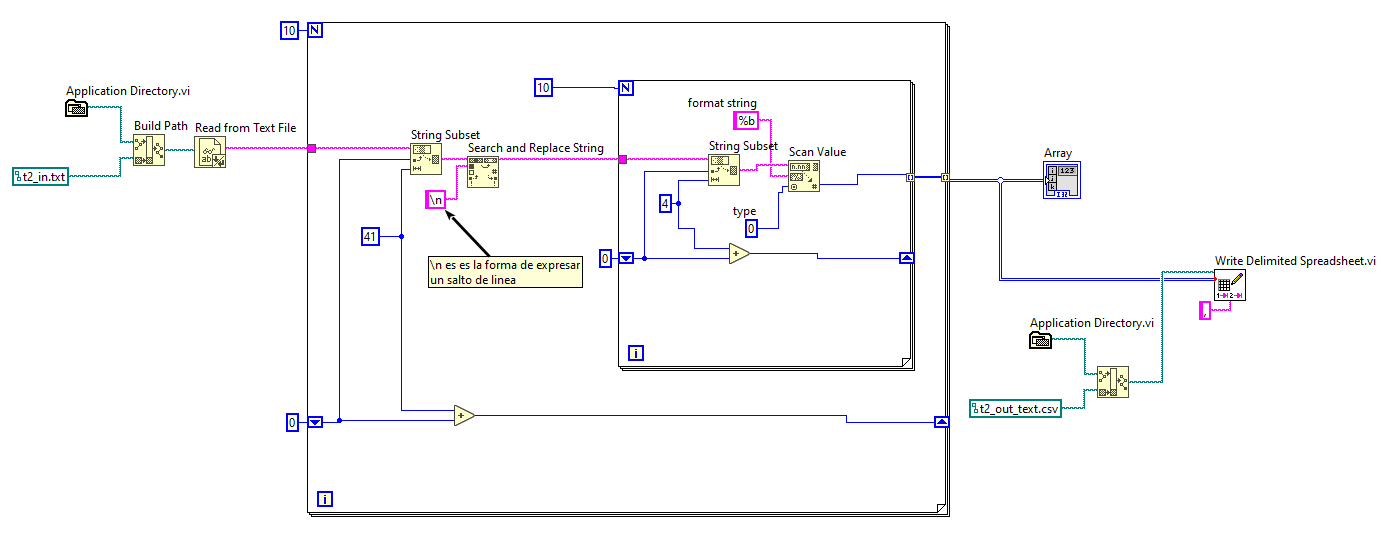
\includegraphics[width=15cm]{fig/t2.1.png}
    \caption{}
    \label{fig:for}
\end{figure}


Usando Simulink realice lo siguiente:

\begin{itemize}
    \item Descargue los archivos \href{https://github.com/juanjorojash/instrumentacion_II/blob/5b8d70f17f7545a45cf6b1aebac0eb5c55f2a2ad/simulaciones/t2.slx}{t2.slx} y \href{https://github.com/juanjorojash/instrumentacion_II/blob/3795263c9e017dead230c0d5c829228d59253f76/simulaciones/t2_process.m}{t2\_process.m} y estúdielos para entender su función.
    \item Modifique el diagrama de bloques de forma que genere un arreglo de cadenas de texto que incluya los números del 0 al 9, las letras de la $A$ a la $Z$ y las letras de la $a$ a la $z$, recuerde modificar el tiempo de la simulación.
    \item Usando \verb+t2_process.m+ genere el archivo \verb+datos.csv+ que contiene el resultado del arreglo separado por comas.
    \item Guarde el diagrama de bloques modificado con el nombre \verb+t2_sol.slx+
    \item Incluya los dos archivos en un archivo comprimido \verb+t2.zip+ y suba al TecDigital
\end{itemize}

Cualquier entrega tardía se califica en base a 70. 


% \bibliographystyle{IEEEtran}
% \bibliography{ref_tareas}

\end{document}